\chapter{Tác dụng dừng và phương trình Euler--Lagrange}

\lectureoverview{Tên quen thuộc \emph{nguyên lý tác dụng tối thiểu} che khuất điểm cốt yếu: quỹ đạo vật lý làm cho tác dụng dừng, nhưng không nhất thiết làm nó nhỏ nhất. Chúng ta sẽ xây dựng mệnh đề ấy từ cân bằng thông thường, mở rộng nó từ các điểm sang toàn bộ các hàm, suy ra phương trình Euler--Lagrange bằng cách rời rạc hóa một đường đi, rồi thu lại các phương trình Newton. Sau đó, tọa độ quay và tọa độ cực sẽ cho thấy vì sao mô tả Lagrange còn hơn cả một sự đổi ký hiệu.}

\section{Dừng, không nhất thiết là nhỏ nhất}

Từ \emph{nhỏ nhất} là phần kém đáng tin của tên gọi truyền thống. Một quỹ đạo cổ điển không phải lúc nào cũng làm cho tác dụng đạt cực tiểu. Thay vào đó, nó có thể cho một cực đại hoặc một điểm yên ngựa trong không gian các quỹ đạo khả dĩ. Nguyên lý đúng là tác dụng là \emph{dừng}: biến thiên bậc nhất của nó triệt tiêu.

Hãy bắt đầu bằng câu hỏi đơn giản hơn về cân bằng. Một hạt vẫn đứng yên thì không có gia tốc, nên hợp lực tác dụng lên nó phải triệt tiêu. Với một lực suy ra từ một thế năng một chiều,
\begin{equation}
  F(x)=-\frac{dV}{dx},
  \label{eq:force-from-v}
\end{equation}
điều kiện cân bằng là
\begin{equation}
  \frac{dV}{dx}=0.
  \label{eq:stationary-v-one}
\end{equation}

\begin{figure}[htbp]
  \centering
  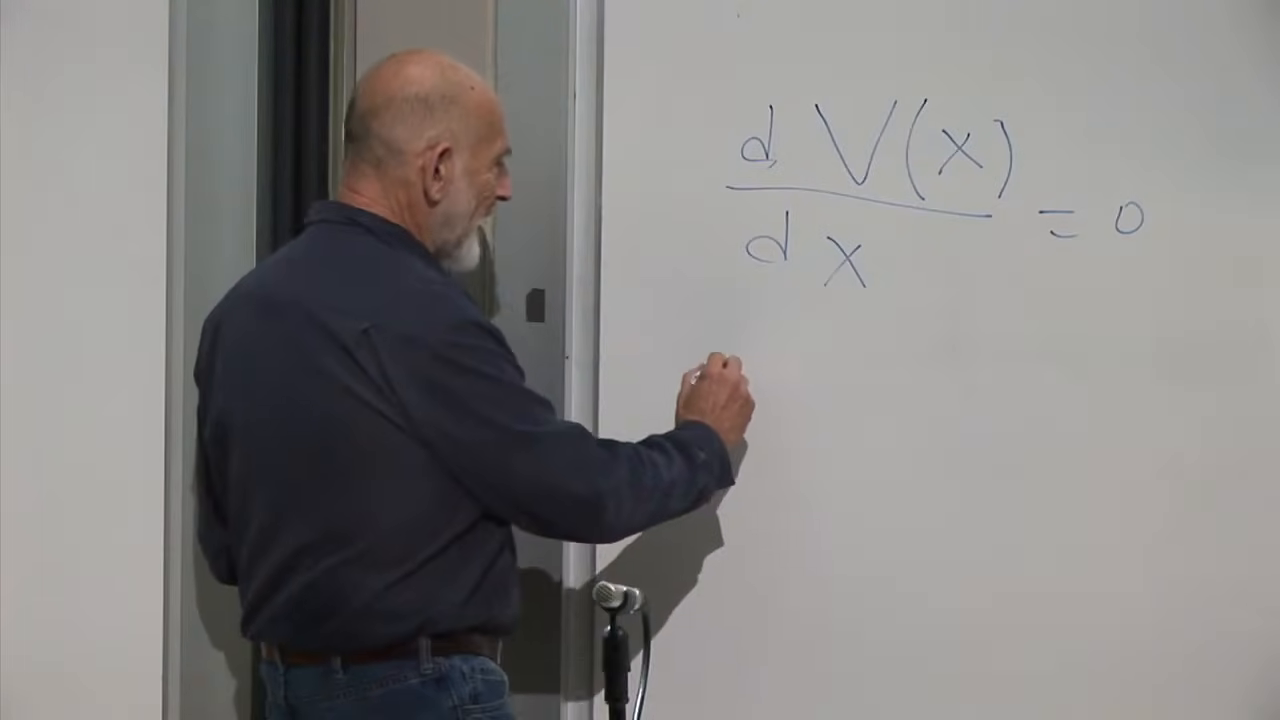
\includegraphics[width=0.74\textwidth]{lecture_03_figure_02.png}
  \caption{Điều kiện cân bằng một chiều: lực triệt tiêu tại điểm mà thế năng dừng.}
  \lectureframe{00:02:51}
\end{figure}

Bây giờ hãy dịch chuyển hạt một lượng nhỏ \(\delta x\). Đến bậc nhất,
\begin{equation}
  \delta V
  =V(x+\delta x)-V(x)
  =\frac{dV}{dx}\,\delta x+O(\delta x^2).
  \label{eq:first-variation-one}
\end{equation}
Ở cân bằng, hạng tuyến tính bằng không với cả hai dấu của \(\delta x\):
\begin{equation}
  \delta V=0
  \qquad\hbox{to first order.}
  \label{eq:delta-v-zero-one}
\end{equation}
Điều này không nói rằng \(V\) hoàn toàn không đổi sau một dịch chuyển hữu hạn. Nó nói rằng biến thiên dẫn đầu là bậc hai hoặc cao hơn. Cả cực tiểu lẫn cực đại đều thỏa mãn điều kiện này.

\begin{figure}[htbp]
  \centering
  \begin{tikzpicture}[scale=0.95,>=Latex]
    \draw[->] (-0.2,0) -- (3.35,0) node[right] {$x$};
    \draw[->] (0,-0.2) -- (0,2.25) node[above] {$V$};
    \draw[blue!65!black,thick,smooth]
      plot coordinates {(0.2,1.85) (0.75,0.85) (1.55,0.35)
                        (2.35,0.85) (3.0,1.85)};
    \fill[red!65!black] (1.55,0.35) circle (2pt);
    \node at (1.55,-0.34) {minimum};
    \begin{scope}[xshift=4.25cm]
      \draw[->] (-0.2,0) -- (3.35,0) node[right] {$x$};
      \draw[->] (0,-0.2) -- (0,2.25) node[above] {$V$};
      \draw[blue!65!black,thick,smooth]
        plot coordinates {(0.2,0.35) (0.75,1.25) (1.55,1.85)
                          (2.35,1.25) (3.0,0.35)};
      \fill[red!65!black] (1.55,1.85) circle (2pt);
      \node at (1.55,-0.34) {maximum};
    \end{scope}
  \end{tikzpicture}
  \caption{Tính dừng cố định đạo hàm bậc nhất, chứ không quyết định điểm đó là cực tiểu hay cực đại.}
  \label{fig:min-max-stationary}
\end{figure}

Với nhiều tọa độ \(q_i\), biến phân bậc nhất là
\begin{equation}
  \delta V
  =\sum_i\frac{\partial V}{\partial q_i}\,\delta q_i.
  \label{eq:first-variation-many}
\end{equation}
Nếu biểu thức này phải triệt tiêu với mọi dịch chuyển vô cùng nhỏ độc lập \(\delta q_i\), thì mọi hệ số đều phải triệt tiêu:
\begin{equation}
  \frac{\partial V}{\partial q_i}=0
  \qquad\hbox{for every }i.
  \label{eq:stationary-v-many}
\end{equation}

Một thế năng hai chiều nên được hình dung như một địa hình đồi núi hơn là như một đường tàu lượn. Một điểm dừng có thể là đáy thung lũng, đỉnh đồi hoặc điểm yên ngựa. Tại một điểm yên ngựa, chuyển động theo một hướng ban đầu đi lên, còn theo một hướng khác ban đầu đi xuống. Vì vậy, tính hồi phục có thể ổn định theo một hướng và không ổn định theo hướng khác, dù mọi đạo hàm bậc nhất đều triệt tiêu ngay tại bản thân điểm đó.

\begin{figure}[htbp]
  \centering
  \includegraphics[width=0.76\textwidth]{lecture_03_figure_06.png}
  \caption{Một điểm yên ngựa là dừng theo mọi hướng bậc nhất, dù các dịch chuyển lân cận tăng theo một trục và giảm theo trục khác.}
  \lectureframe{00:08:20}
\end{figure}

Trong một không gian với nhiều tọa độ, các điểm yên ngựa điển hình hơn các cực đại hoặc cực tiểu thuần túy. Đó là lý do từ \emph{dừng} mới là từ đáng tin cậy. Điều kiện
\begin{equation}
  \delta V=0
  \label{eq:equilibrium-variation}
\end{equation}
tóm tắt trạng thái cân bằng mà không phán định trước hành vi bậc hai.

\section{Từ các điểm đến các hàm}

Cơ học quan tâm đến toàn bộ chuyển động, chứ không phải các điểm cân bằng cô lập. Một quỹ đạo là một hàm như \(x(t)\), hoặc một bộ \((x(t),y(t),z(t))\). Bài toán toán học về việc làm cho một đại lượng dừng bằng cách biến thiên cả một hàm được gọi là \emph{phép tính biến phân}. Trước khi áp dụng nó cho chuyển động, hãy xét 3 ví dụ đơn giản hơn.

\subsection{Các đường cong ngắn nhất và đường trắc địa}

Cố định hai điểm trong mặt phẳng và biểu diễn một đường cong nối giữa chúng bằng \(y(x)\). Trên một đoạn ngắn,
\begin{equation}
  ds=\sqrt{dx^2+dy^2}
  =dx\sqrt{1+\left(\frac{dy}{dx}\right)^2},
  \label{eq:line-element}
\end{equation}
trong đó dạng cuối cùng giả sử \(dx>0\). Tổng độ dài là phiếm hàm
\begin{equation}
  S[y]=\int_{x_0}^{x_1}
  \sqrt{1+y'(x)^2}\,dx.
  \label{eq:arc-length-functional}
\end{equation}
Dấu ngoặc vuông nhấn mạnh rằng \(S\) nhận cả một hàm làm đầu vào. Đường thẳng được chọn bởi điều kiện
\begin{equation}
  \delta S=0
  \label{eq:stationary-length}
\end{equation}
dưới những biến đổi nhỏ của đường cong nhưng vẫn giữ cố định cả hai đầu mút.

\begin{figure}[htbp]
  \centering
  \includegraphics[width=0.78\textwidth]{lecture_03_figure_07.png}
  \caption{Một đường cong thử giữa hai đầu mút cố định. Độ dài của nó là tổng các cạnh huyền vi phân \(ds\).}
  \lectureframe{00:13:36}
\end{figure}

Cùng câu hỏi ấy cũng có thể được đặt ra trên một mặt cong. Hình ảnh vật lý về con đường bị ràng buộc ngắn nhất là kéo căng một sợi dây giữa hai cọc. Một đường cong có độ dài dừng như vậy là một \emph{đường trắc địa}. Trên một mặt phẳng, nó là đường thẳng; trên mặt cầu hoặc mặt đồi núi thì nói chung không phải vậy.

\subsection{Nguyên lý Fermat}

Một tia sáng trong một môi trường mà tốc độ phụ thuộc vị trí \(c(x,y)\) không nhất thiết đi theo đường đi ngắn nhất trong không gian. Thời gian cần cho một đoạn nhỏ bằng quãng đường chia cho tốc độ cục bộ, nên
\begin{equation}
  T[y]
  =\int_{x_0}^{x_1}
  \frac{\sqrt{1+y'(x)^2}}{c(x,y)}\,dx.
  \label{eq:fermat-functional}
\end{equation}
Nguyên lý Fermat đòi hỏi
\begin{equation}
  \delta T=0.
  \label{eq:fermat-stationary}
\end{equation}
Khi \(c\) không đổi, điều này quy về bài toán khoảng cách ngắn nhất. Tuy nhiên, trong một môi trường khúc xạ biến thiên, đường đi nhanh nhất là sự cân bằng giữa quãng đường và tốc độ truyền cục bộ.

\begin{figure}[htbp]
  \centering
  \includegraphics[width=0.80\textwidth]{lecture_03_figure_08.png}
  \caption{Phiếm hàm thời gian ngắn nhất cho một tia trong một môi trường mà tốc độ ánh sáng cục bộ phụ thuộc vào vị trí.}
  \lectureframe{00:22:50}
\end{figure}

Một trò đùa thời sự nhắc đến tuyên bố khi ấy còn mới rằng neutrino chuyển động nhanh bất thường ở Italy. Lập luận vật lý lập tức quay lại ví dụ đáng tin cậy hơn: ánh sáng thông thường thay đổi tốc độ trong vật liệu theo chiết suất.

\subsection{Một dây xích treo}

Một dây xích được ghim tại hai điểm sẽ ổn định thành một đường dây xích. Mỗi mẩu nhỏ đóng góp thế năng hấp dẫn, nên tổng thế năng bản thân nó chính là một tích phân trên dây xích. Một lần nữa, các đầu mút là cố định, hình dạng chưa biết là một hàm, và một tích phân phải dừng.

\begin{figure}[htbp]
  \centering
  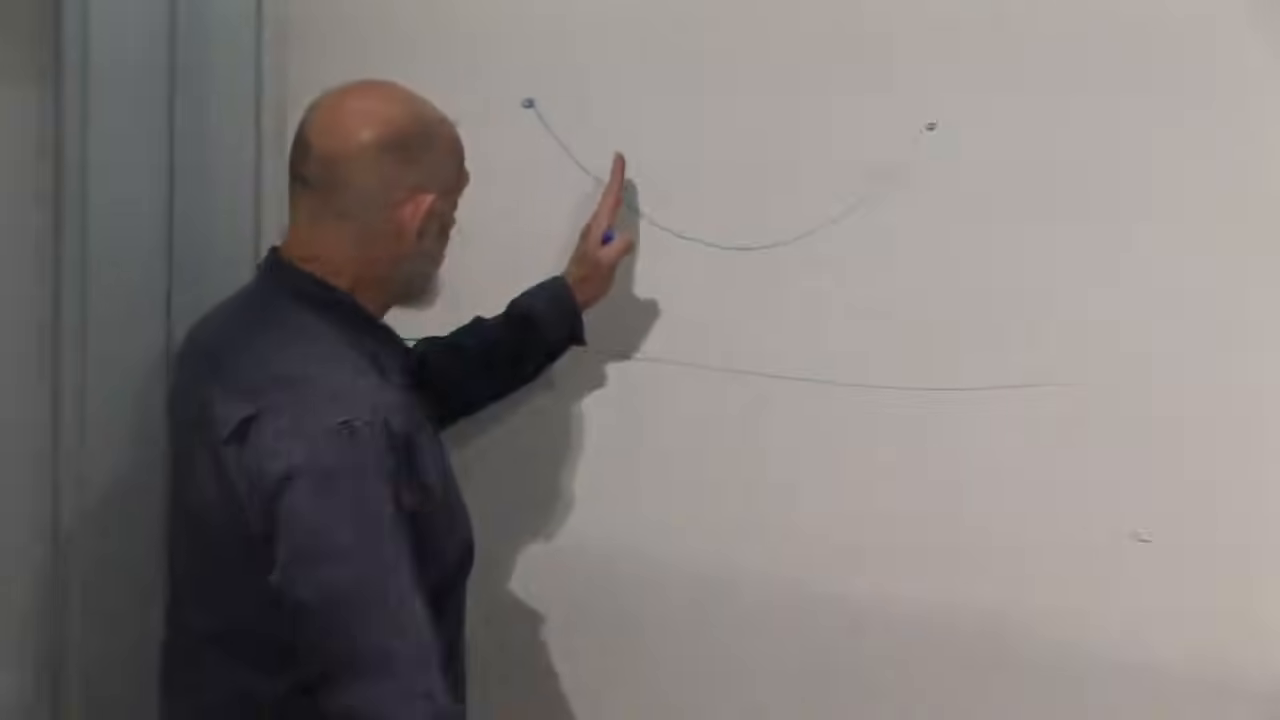
\includegraphics[width=0.76\textwidth]{lecture_03_figure_03.png}
  \caption{Một dây xích treo giữa các giá đỡ cố định. Hình dạng dừng của nó được xác định bởi tổng thế năng hấp dẫn.}
  \lectureframe{00:30:41}
\end{figure}

Các ví dụ này có cùng một cấu trúc: hai đầu mút cố định, một hàm ở giữa chúng, và một tích phân mà biến phân bậc nhất của nó triệt tiêu. Rút gọn một chỉ dẫn toàn cục như vậy thành một phương trình vi phân chính là ý nghĩa của việc giải bài toán biến phân.

\section{Cơ học như một bài toán giá trị biên}

Một quỹ đạo thường được vẽ với thời gian nằm ngang vì \(t\) là biến độc lập. Tuy vậy, trong vật lý vẫn có một quy ước rất mạnh là vẽ thời gian hướng lên trên. Một đoạn xen kể lại các thí nghiệm trong đó người ta sắp xếp các bức hình từ trẻ đến già theo những hướng gắn với hệ chữ viết của mình: người đọc từ trái sang phải có xu hướng xếp từ trái sang phải, người đọc từ phải sang trái thì ngược lại, còn người được rèn theo chiều dọc thì xếp theo chiều dọc. Trò đùa kết luận rằng các nhà vật lý là những người khăng khăng cho rằng thời gian chảy lên trên. Ở đây ta sẽ dùng trục \(t\) nằm ngang theo quy ước thông thường vì như vậy \(x(t)\) được đọc một cách tự nhiên như một đồ thị.

Trong mô tả giá trị đầu, dữ liệu tại \(t_0\) là
\begin{equation}
  x(t_0)=x_0,
  \qquad
  \dot x(t_0)=v_0.
  \label{eq:initial-value-data}
\end{equation}
Khi đó, phương trình Newton xác định quỹ đạo tiếp theo. Một mô tả biến phân đặt ra một bài toán khác: cho trước hai sự kiện ở hai đầu mút,
\begin{equation}
  x(t_0)=x_0,
  \qquad
  x(t_1)=x_1,
  \label{eq:boundary-value-data}
\end{equation}
rồi xác định đường đi vật lý giữa chúng. Vận tốc đầu không còn được cho sẵn nữa; nó trở thành một phần của nghiệm.

\begin{figure}[htbp]
  \centering
  \includegraphics[width=0.76\textwidth]{lecture_03_figure_09.png}
  \caption{Một quỹ đạo cơ học \(x(t)\). Ta có thể cho trước vị trí và độ dốc ở một đầu, hoặc các vị trí tại hai thời điểm đầu mút.}
  \lectureframe{00:27:41}
\end{figure}

Đại lượng cần được làm cho dừng là \emph{tác dụng},
\begin{equation}
  A[x]=\int_{t_0}^{t_1}L(x,\dot x,t)\,dt.
  \label{eq:action-one}
\end{equation}
Hàm dưới dấu tích phân \(L\) là \emph{hàm Lagrange}. Nó có thể phụ thuộc vào vị trí, vận tốc và phụ thuộc tường minh vào thời gian. Nguyên lý tác dụng là
\begin{equation}
  \delta A=0
  \label{eq:stationary-action}
\end{equation}
đối với mọi biến thiên nhỏ của quỹ đạo thỏa
\begin{equation}
  \delta x(t_0)=\delta x(t_1)=0.
  \label{eq:fixed-endpoint-variations}
\end{equation}
Điều kiện ở đầu mút là thiết yếu: ta so sánh các quỹ đạo lân cận nối cùng hai sự kiện.

\section{Một phép suy dẫn rời rạc của phương trình Euler--Lagrange}

Tác dụng là một phiếm hàm của vô số giá trị của quỹ đạo. Để làm cho biến thiên của nó trở nên cụ thể, hãy chia khoảng thời gian thành các bước có độ dài \(\epsilon\),
\begin{equation}
  t_n=t_0+n\epsilon,
  \qquad
  x_n=x(t_n),
  \label{eq:discrete-times}
\end{equation}
và xấp xỉ vận tốc trên khoảng thứ \(n\) bằng
\begin{equation}
  v_n=\frac{x_{n+1}-x_n}{\epsilon}.
  \label{eq:discrete-velocity}
\end{equation}
Tích phân trở thành tổng thông thường
\begin{equation}
  A_\epsilon
  =\sum_{n=0}^{N-1}
  \epsilon L\left(x_n,\frac{x_{n+1}-x_n}{\epsilon}\right).
  \label{eq:discrete-action}
\end{equation}
Ta dùng \(n\) làm nhãn cho lát thời gian để \(i\) còn có thể dùng sau này cho các tọa độ không gian và các hạt.

\begin{figure}[htbp]
  \centering
  \includegraphics[width=0.82\textwidth]{lecture_03_figure_10.png}
  \caption{Quỹ đạo được thay bằng một chuỗi các lát thời gian. Biến đổi một độ cao bên trong chỉ làm thay đổi hai đoạn lân cận của nó.}
  \lectureframe{00:38:30}
\end{figure}

Hãy biến thiên một điểm bên trong \(x_n\), đồng thời giữ cố định mọi \(x_k\) khác. Chỉ có 2 hạng trong tổng phụ thuộc vào \(x_n\):
\begin{align}
  A_\epsilon\big|_{x_n}
  &=
  \epsilon L\left(x_n,\frac{x_{n+1}-x_n}{\epsilon}\right)
  \notag\\
  &\quad+
  \epsilon L\left(x_{n-1},
                  \frac{x_n-x_{n-1}}{\epsilon}\right).
  \label{eq:two-neighbor-terms}
\end{align}
Lấy đạo hàm cho
\begin{align}
  0=\frac{\partial A_\epsilon}{\partial x_n}
  &=
  \epsilon\frac{\partial L_n}{\partial x_n}
  -\frac{\partial L_n}{\partial v_n}
  +\frac{\partial L_{n-1}}{\partial v_{n-1}}.
  \label{eq:discrete-el-variation}
\end{align}
Các dấu ngược nhau có nguồn gốc hình học đơn giản. Nâng \(x_n\) lên làm tăng độ dốc của khoảng ở phía sau nó và làm giảm độ dốc của khoảng ở phía trước nó.

\begin{figure}[htbp]
  \centering
  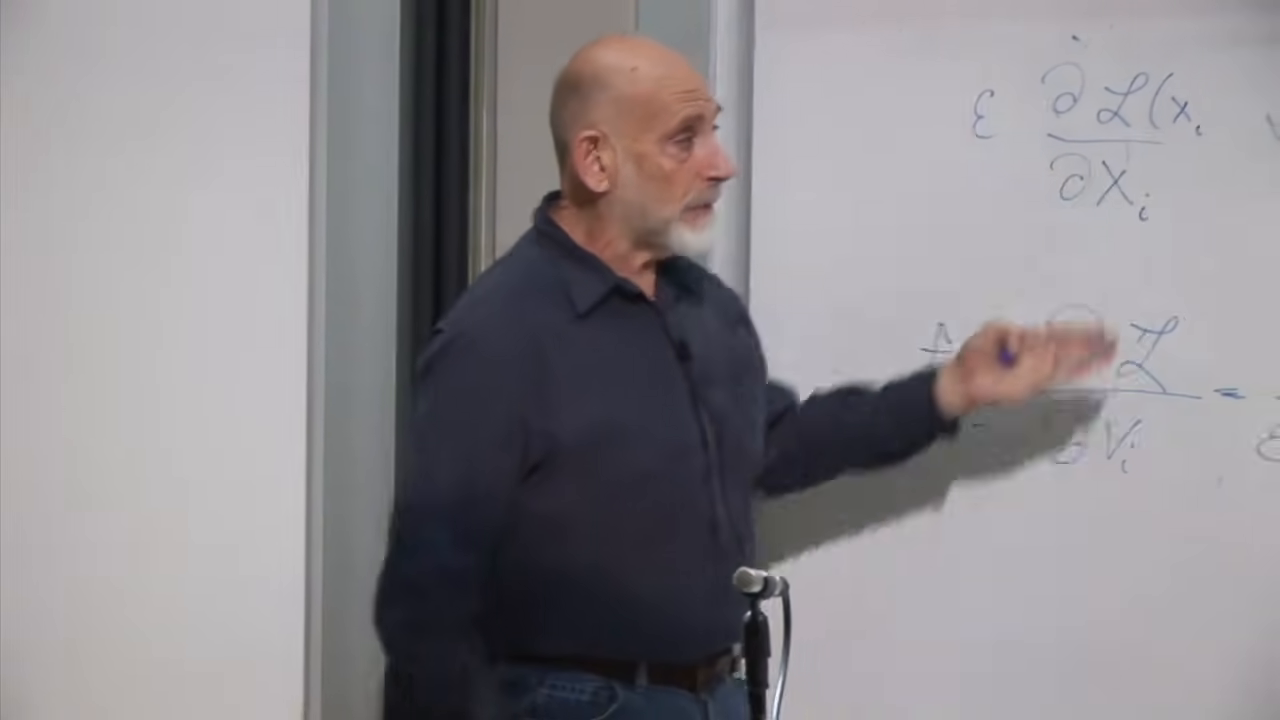
\includegraphics[width=0.74\textwidth]{lecture_03_figure_04.png}
  \caption{Đạo hàm trực tiếp theo vị trí và hai đóng góp từ đạo hàm theo vận tốc của các đoạn lân cận trong biến phân rời rạc.}
  \lectureframe{00:45:26}
\end{figure}

Sắp xếp lại phương trình ~\eqref{eq:discrete-el-variation}:
\begin{equation}
  \frac{1}{\epsilon}
  \left(
    \frac{\partial L_n}{\partial v_n}
    -\frac{\partial L_{n-1}}{\partial v_{n-1}}
  \right)
  =
  \frac{\partial L_n}{\partial x_n}.
  \label{eq:discrete-el}
\end{equation}
Vế trái là một thương sai phân giữa các điểm lân cận. Khi \(\epsilon\to0\), đường gấp khúc trở thành một quỹ đạo trơn và thương đó trở thành đạo hàm theo thời gian:
\begin{equation}
  \boxed{
  \frac{d}{dt}\left(\frac{\partial L}{\partial\dot x}\right)
  =
  \frac{\partial L}{\partial x}}
  .
  \label{eq:euler-lagrange-one}
\end{equation}
Đây là phương trình Euler--Lagrange.

\begin{figure}[htbp]
  \centering
  \includegraphics[width=0.78\textwidth]{lecture_03_figure_11.png}
  \caption{Phương trình Euler--Lagrange hoàn chỉnh thu được từ điều kiện dừng tại mọi lát thời gian bên trong.}
  \lectureframe{00:49:25}
\end{figure}

Một khi \(L\) đã được chỉ rõ, phương trình ~\eqref{eq:euler-lagrange-one} hoạt động như một cỗ máy: lấy đạo hàm của hàm đã cho, và cỗ máy trả về một phương trình vi phân cho quỹ đạo.

\begin{classroomqa}
  \audiencequestion{Liệu kết quả Euler--Lagrange có đúng với mọi hàm của \(x\) và \(\dot x\) không?\lecturetimestamp{00:49:37--00:50:24}}
  \lecturerresponse{Có, với điều kiện có đủ tính chính quy để lấy các đạo hàm. Ví dụ độ dài cung có đúng cùng dạng sau khi đổi nhãn biến độc lập của nó \(x\) thành vai trò do \(t\) đảm nhiệm, và hàm chưa biết của nó \(y(x)\) thành vai trò do \(x(t)\) đảm nhiệm. Phương trình Euler--Lagrange của nó có nghiệm là các đường thẳng.}
\end{classroomqa}

\section{Các phương trình Newton từ hàm Lagrange}

Đối với một hạt chuyển động trên một đường thẳng trong một thế \(V(x)\), lấy
\begin{equation}
  L(x,\dot x)=T-V
  =\frac12m\dot x^2-V(x).
  \label{eq:lagrangian-tv-one}
\end{equation}
Dấu trừ có thể trông lạ vì tổng năng lượng là \(T+V\). Nhưng hàm Lagrange không phải là năng lượng. Tiêu chuẩn kiểm tra nó là liệu cỗ máy Euler--Lagrange có trả về đúng chuyển động hay không. Một cuộc bỏ phiếu giả về dấu bị từ chối: đáp án phải được kiểm tra, chứ không phải được bầu chọn.

Trước hết,
\begin{equation}
  \frac{\partial L}{\partial\dot x}=m\dot x.
  \label{eq:conjugate-momentum-one}
\end{equation}
Đây là động lượng. Tổng quát hơn, động lượng liên hợp với bất kỳ tọa độ nào \(q\) được định nghĩa bởi
\begin{equation}
  p_q=\frac{\partial L}{\partial\dot q}.
  \label{eq:conjugate-momentum-general}
\end{equation}
Lấy đạo hàm theo thời gian của phương trình ~\eqref{eq:conjugate-momentum-one} cho \(m\ddot x\), còn
\begin{equation}
  \frac{\partial L}{\partial x}
  =-\frac{dV}{dx}.
  \label{eq:lagrangian-position-derivative}
\end{equation}
Vì thế, phương trình Euler--Lagrange là
\begin{equation}
  m\ddot x=-\frac{dV}{dx}=F(x),
  \label{eq:newton-from-action}
\end{equation}
đó chính là định luật thứ hai của Newton.

\begin{figure}[htbp]
  \centering
  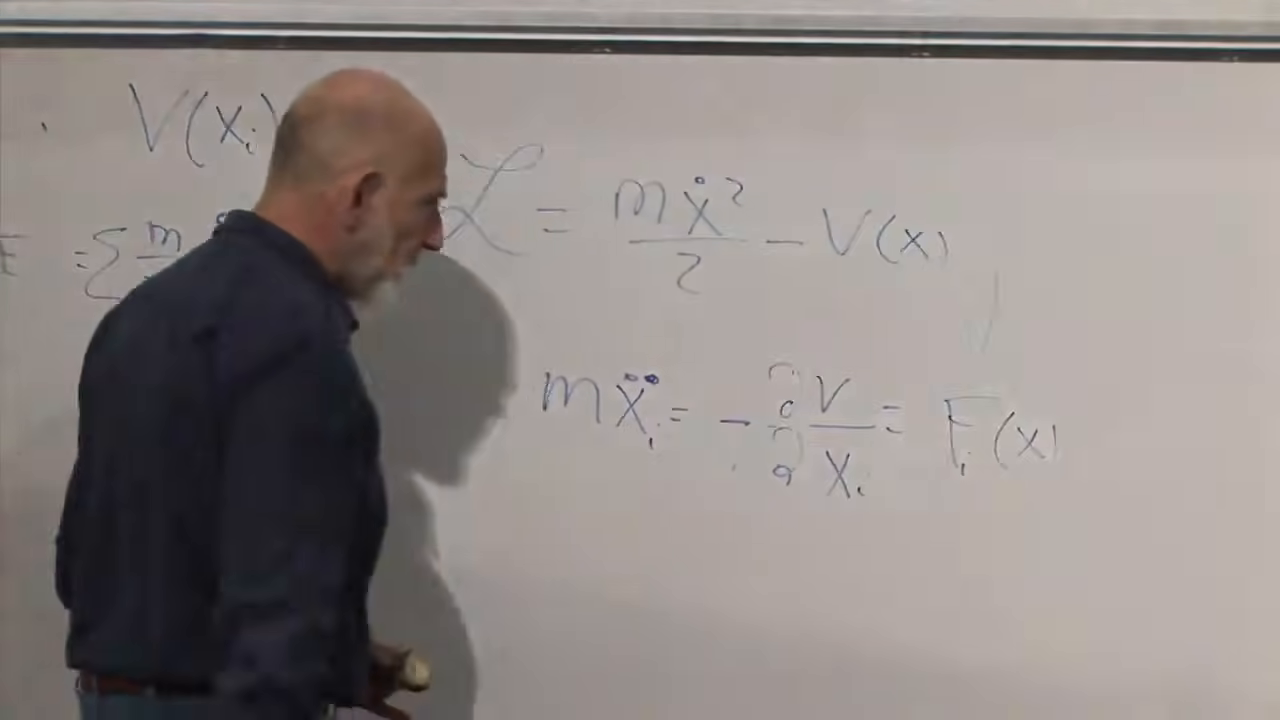
\includegraphics[width=0.80\textwidth]{lecture_03_figure_05.png}
  \caption{Động năng, thế năng, \(L=T-V\), và dạng theo thành phần của phương trình Newton được phục hồi trên cùng một bảng.}
  \lectureframe{00:57:52}
\end{figure}

Với nhiều tọa độ \(q_i\),
\begin{equation}
  L(\mathbf q,\dot{\mathbf q})
  =\sum_i\frac12m_i\dot q_i^{\,2}-V(q_1,q_2,\ldots),
  \label{eq:lagrangian-tv-many}
\end{equation}
và có một phương trình cho mỗi tọa độ:
\begin{equation}
  \frac{d}{dt}\left(\frac{\partial L}{\partial\dot q_i}\right)
  =\frac{\partial L}{\partial q_i}
  \quad\Longrightarrow\quad
  m_i\ddot q_i=-\frac{\partial V}{\partial q_i}=F_i.
  \label{eq:euler-lagrange-many}
\end{equation}
Quỹ đạo vẫn là một đường cong duy nhất, nay đi qua một không gian cấu hình nhiều chiều.

\begin{classroomqa}
  \audiencequestion{Chẳng lẽ ta chỉ đơn thuần đi ngược từ định luật Newton rồi thiết kế một phiếm hàm tái tạo ra đáp án?\lecturetimestamp{00:58:07--01:00:04}}
  \lecturerresponse{Đó không phải là cách nhìn hữu ích. Hàm Lagrange là mô tả cô đọng của hệ vật lý: một hàm của mọi tọa độ và vận tốc gói gọn toàn bộ các phương trình chuyển động của nó. Trong các lý thuyết mới, các nhà vật lý thường đề xuất một tác dụng rồi suy ra các phương trình, thay vì đoán riêng từng phương trình.}
\end{classroomqa}

Sự gói gọn đó là một ưu điểm. Tự do tọa độ là một ưu điểm khác. Mệnh đề rằng một đường thẳng là ngắn nhất không phụ thuộc vào việc mặt phẳng được mô tả bằng tọa độ Descartes, tọa độ cực hay tọa độ cong. Tương tự, tính dừng của tác dụng là độc lập với tọa độ, dù công thức cho \(L\) và các phương trình theo thành phần thu được có thay đổi.

\section{Một hạt tự do nhìn từ đu quay}

Gọi \((x,y)\) là các tọa độ Descartes trong hệ quán tính và để \((X,Y)\) quay đều với vận tốc góc \(\omega\). Theo quy ước định hướng dùng ở đây, \begin{align}
  x&=X\cos\omega t+Y\sin\omega t,
  \notag\\
  y&=-X\sin\omega t+Y\cos\omega t.
  \label{eq:rotating-coordinate-map}
\end{align} Góc giữa hai hệ trục là \(\omega t\).

\begin{figure}[htbp]\centering
  \includegraphics[width=0.76\textwidth]{lecture_03_figure_12.png}\caption{Các trục Descartes quán tính và quay đều. Cùng một điểm được gán các tọa độ quay phụ thuộc thời gian.}\lectureframe{01:06:05}\end{figure}

Một hạt tự do có Lagrangian trong hệ quán tính là \begin{equation}
  L_{\mathrm{in}}
  =\frac{m}{2}\left(\dot x^2+\dot y^2\right).
  \label{eq:free-inertial-lagrangian}
\end{equation} Lấy đạo hàm phương trình~\eqref{eq:rotating-coordinate-map} và dùng \(\sin^2\omega t+\cos^2\omega t=1\). Các hạng lượng giác gộp lại thành \begin{align}
  \dot x^2+\dot y^2
  &=
  \dot X^2+\dot Y^2\\
  &\quad+\omega^2(X^2+Y^2)\\
  &\quad+2\omega(Y\dot X-X\dot Y).
  \label{eq:rotating-speed}
\end{align} Do đó \begin{align}
  L_{\mathrm{rot}}
  &=
  \frac{m}{2}(\dot X^2+\dot Y^2)\\
  &\quad+\frac{m\omega^2}{2}(X^2+Y^2)\\
  &\quad+m\omega(Y\dot X-X\dot Y).
  \label{eq:rotating-lagrangian}
\end{align}

\begin{figure}[htbp]\centering
  \includegraphics[width=0.84\textwidth]{lecture_03_figure_13.png}\caption{Lagrangian đã biến đổi của hạt tự do: động năng thông thường, một hạng ly tâm bậc hai và một hạng tuyến tính theo vận tốc.}\lectureframe{01:12:16}\end{figure}

Hạng bậc hai theo tọa độ có dạng \(-V_{\mathrm{fict}}\), trong đó \begin{equation}
  V_{\mathrm{fict}}
  =-\frac{m\omega^2}{2}(X^2+Y^2).
  \label{eq:centrifugal-potential}
\end{equation} Nó giảm khi đi ra ngoài, nên sinh ra lực ly tâm \(m\omega^2(X,Y)\).

Hạng cuối trong phương trình~\eqref{eq:rotating-lagrangian} tuyến tính theo cả tọa độ lẫn vận tốc. Áp dụng phương trình Euler--Lagrange cho ta \begin{align}
  m\ddot X&=m\omega^2X-2m\omega\dot Y,
  \notag\\
  m\ddot Y&=m\omega^2Y+2m\omega\dot X.
  \label{eq:rotating-equations}
\end{align} Các hạng tỉ lệ với \(\omega^2\) là ly tâm; còn các hạng tỉ lệ với vận tốc là Coriolis. Dưới dạng vectơ trong mặt phẳng quay, \begin{equation}
  \mathbf F_{\mathrm{C}}
  =-2m\,\boldsymbol\omega\times\mathbf v_{\mathrm{rot}},
  \label{eq:coriolis-vector}
\end{equation} với dấu được điều chỉnh nếu chọn quy ước định hướng ngược lại.

\begin{figure}[htbp]\centering
  \includegraphics[width=0.84\textwidth]{lecture_03_figure_14.png}\caption{Các phương trình trong hệ quay, trong đó các hạng tỉ lệ với tọa độ cho gia tốc ly tâm còn các hạng chéo theo vận tốc cho gia tốc Coriolis.}\lectureframe{01:20:20}\end{figure}

Vấn đề không phải là phép tính đại số biến mất. Mà là một phép biến đổi tọa độ của một hàm vô hướng duy nhất sinh ra đồng thời cả hai phương trình ghép cặp lẫn cả hai lực hư cấu.

\begin{classroomqa}\audiencequestion{Phương pháp này có áp dụng được cho các tọa độ cong tùy ý không?\lecturetimestamp{01:22:01--01:22:17}}\lecturerresponse{Có. Các tọa độ mới có thể là cong, và thậm chí còn có thể phụ thuộc tường minh vào thời gian, như các tọa độ quay. Viết lại tác dụng theo các biến mới rồi áp dụng cùng một quy tắc Euler--Lagrange.}\end{classroomqa}

\section{Tọa độ cực và một góc tuần hoàn}

Đối với tọa độ cực thông thường, \begin{equation}
  x=r\cos\theta,
  \qquad
  y=r\sin\theta.
  \label{eq:polar-map}
\end{equation} Cả \(r\) lẫn \(\theta\) đều có thể biến thiên theo thời gian. Lấy đạo hàm rồi cộng các bình phương lại, ta được \begin{equation}
  \dot x^2+\dot y^2
  =\dot r^2+r^2\dot\theta^2.
  \label{eq:polar-speed}
\end{equation} Với một thế năng tâm \(V(r)\), \begin{equation}
  L
  =\frac{m}{2}\left(\dot r^2+r^2\dot\theta^2\right)-V(r).
  \label{eq:polar-lagrangian}
\end{equation}

\begin{figure}[htbp]\centering
  \includegraphics[width=0.80\textwidth]{lecture_03_figure_15.png}\caption{Hình học cực và sự phân tách động năng thành chuyển động theo bán kính và chuyển động góc.}\lectureframe{01:23:30}\end{figure}

Phương trình bán kính là \begin{equation}
  m\ddot r
  =mr\dot\theta^2-\frac{dV}{dr}.
  \label{eq:radial-equation}
\end{equation} Hạng thứ nhất là phần đóng góp ly tâm hướng ra ngoài gắn với chuyển động góc của chính hạt.

Đối với góc, \begin{equation}
  \frac{d}{dt}\left(\frac{\partial L}{\partial\dot\theta}\right)
  =\frac{\partial L}{\partial\theta}=0,
  \label{eq:theta-el}
\end{equation} vì thế năng tâm không phụ thuộc tường minh vào \(\theta\). Do đó \begin{equation}
  \frac{d}{dt}\left(mr^2\dot\theta\right)=0,
  \qquad
  mr^2\dot\theta=\ell,
  \label{eq:angular-momentum}
\end{equation} trong đó \(\ell\) là mômen động lượng được bảo toàn.

\begin{figure}[htbp]\centering
  \includegraphics[width=0.82\textwidth]{lecture_03_figure_16.png}\caption{Phương trình Euler--Lagrange cho biến góc có vế phải bằng không, qua đó bộc lộ sự bảo toàn của \(mr^2\dot\theta\).}\lectureframe{01:29:25}\end{figure}

Phương trình góc cho \begin{equation}
  \dot\theta=\frac{\ell}{mr^2}.
  \label{eq:theta-dot-angular-momentum}
\end{equation} Thế vào phương trình~\eqref{eq:radial-equation} thì còn lại một phương trình duy nhất cho \(r\): \begin{equation}
  m\ddot r
  =\frac{\ell^2}{mr^3}-\frac{dV}{dr}.
  \label{eq:effective-radial-equation}
\end{equation}

Một tọa độ không xuất hiện trong \(L\) theo truyền thống được gọi là \emph{tuần hoàn}, ngay cả khi nó không phải là một góc. Nếu \(q\) là tuần hoàn, thì \begin{equation}
  \frac{\partial L}{\partial q}=0
  \quad\Longrightarrow\quad
  \frac{d}{dt}\left(\frac{\partial L}{\partial\dot q}\right)=0.
  \label{eq:cyclic-conservation}
\end{equation} Xung lượng liên hợp của nó được bảo toàn. Đây là thoáng thấy đầu tiên về mối liên hệ tổng quát giữa đối xứng và định luật bảo toàn.

\section{Những câu hỏi về ý nghĩa, năng lượng và phạm vi}

Những câu hỏi sau đây cho thấy nội dung sâu hơn của hình thức này nằm ở đâu.

\begin{classroomqa}\audiencequestion{Có lý do độc lập nào để đi đến Lagrangian, ngoài việc phát hiện ra rằng nó cho các phương trình cổ điển đúng không?\lecturetimestamp{01:33:25--01:35:07}}\lecturerresponse{Về mặt lịch sử, hơn một thế kỷ cơ học cổ điển đã cho thấy rằng hạt, sóng và trường điện từ đều có thể được viết dưới dạng này. Ở cấp độ cổ điển, thành công tích lũy ấy là một sự kiện thực nghiệm về cách các định luật được tổ chức. Lời giải thích sâu hơn đến từ cơ học lượng tử và sẽ được để lại về sau.}\end{classroomqa}

\begin{classroomqa}\audiencequestion{Trong Lagrangian của hệ quay, có thể gán hạng tuyến tính theo vận tốc cho một động năng hoặc thế năng thông thường không?\lecturetimestamp{01:35:08--01:36:23}}\lecturerresponse{Không. Đại lượng bảo toàn gắn với tịnh tiến theo thời gian được thu được bằng phép xây dựng Hamiltonian, chứ không phải bằng cách đọc mọi hạng trong \(L\) như động năng hoặc thế năng. Đối với phương trình~\eqref{eq:rotating-lagrangian}, hạng tuyến tính theo vận tốc bị triệt tiêu khỏi \(\sum_a\dot q_a\,\partial L/\partial\dot q_a-L\). Cách xử lý Hamiltonian sẽ sắp xếp điều này một cách hệ thống.}\end{classroomqa}

Quả thật, vì \(L_{\mathrm{rot}}\) không phụ thuộc tường minh vào thời gian, \begin{equation}
  \begin{aligned}
    H_{\mathrm{rot}}
    &=\dot X\frac{\partial L}{\partial\dot X}
     +\dot Y\frac{\partial L}{\partial\dot Y}-L\\
    &=\frac{m}{2}(\dot X^2+\dot Y^2)
     -\frac{m\omega^2}{2}(X^2+Y^2)
  \end{aligned}
  \label{eq:rotating-hamiltonian-preview}
\end{equation} được bảo toàn. Đó là tích phân Jacobi trong hệ quay, không phải cùng một trị số năng lượng mà người quan sát quán tính gán. Các phép đổi tọa độ phụ thuộc thời gian không nhất thiết giữ nguyên dạng số của năng lượng.

\begin{classroomqa}\audiencequestion{Nếu một quỹ đạo cong là do hấp dẫn gây ra thì sao?\lecturetimestamp{01:36:30--01:37:10}}\lecturerresponse{Đối với hấp dẫn Newton, chỉ cần dùng \(V(r)=-GMm/r\) trong Lagrangian lực tâm. Không-thời gian cong thuộc thuyết tương đối rộng và không được giả định ở đây.}\end{classroomqa}

\begin{classroomqa}\audiencequestion{Thế ly tâm và năng lượng của nó có chỉ là hư cấu thôi không?\lecturetimestamp{01:37:13--01:40:14}}\lecturerresponse{Người quan sát trên bệ quay đo được các lực hiệu dụng và có thể một cách nhất quán dùng đại lượng bảo toàn trong hệ quay. \emph{Hư cấu} có nghĩa là những hạng này phát sinh từ một mô tả phi quán tính, chứ không phải rằng các hiệu ứng quan sát được của chúng là tưởng tượng. Bản thân năng lượng không bất biến dưới một phép đổi tọa độ tổng quát phụ thuộc thời gian.}\end{classroomqa}

\begin{classroomqa}\audiencequestion{Lực Coriolis phụ thuộc vận tốc hướng theo hướng nào?\lecturetimestamp{01:40:22--01:42:36}}\lecturerresponse{Nó vuông góc với vận tốc trong hệ quay, với độ lớn tỉ lệ với tốc độ và với vận tốc góc của hệ. Trong mặt phẳng, các thành phần hoán đổi \(\dot X\) và \(\dot Y\) với dấu trái ngược, như trong phương trình~\eqref{eq:rotating-equations}.}\end{classroomqa}

\begin{figure}[htbp]\centering
  \includegraphics[width=0.76\textwidth]{lecture_03_figure_17.png}\caption{Mẫu thành phần chéo theo vận tốc: lực Coriolis vuông góc với vận tốc trong hệ quay.}\lectureframe{01:41:40}\end{figure}

\begin{classroomqa}\audiencequestion{Lagrangian xuất phát có bắt buộc phải được viết trong một hệ quán tính không?\lecturetimestamp{01:42:37--01:44:00}}\lecturerresponse{Đối với một hạt tự do thông thường, định luật của Newton trong hệ quán tính cung cấp dạng khởi đầu đơn giản \(m(\dot x^2+\dot y^2)/2\). Một khi định luật vật lý ấy đã được biết, tác dụng có thể được biến đổi sang bất kỳ tọa độ nào khác. Không nên một cách độc lập giả định cùng công thức động năng đơn giản ấy trong một hệ quay.}\end{classroomqa}

Cùng kiểu hạng tuyến tính theo vận tốc cũng xuất hiện đối với một hạt tích điện trong từ trường: \begin{equation}
  L_{\mathrm{em}}
  =\frac12m\mathbf v^2
   +q\mathbf A(\mathbf r,t)\cdot\mathbf v
   -q\phi(\mathbf r,t).
  \label{eq:electromagnetic-lagrangian}
\end{equation} Đối với một từ trường đều vuông góc với mặt phẳng, chuẩn đối xứng \(\mathbf A=\tfrac12\mathbf B\times\mathbf r\) tạo ra một hạng tỉ lệ với \(X\dot Y-Y\dot X\), có cùng cấu trúc đại số với hạng Coriolis.

\begin{figure}[htbp]\centering
  \includegraphics[width=0.82\textwidth]{lecture_03_figure_18.png}\caption{Hạng của hệ quay tuyến tính theo vận tốc gợi ra sự so sánh với một hạt tích điện trong từ trường đều.}\lectureframe{01:44:40}\end{figure}

\begin{classroomqa}\audiencequestion{Ngoài tính trơn, có những ràng buộc nào đối với việc hàm nào có thể đóng vai trò một Lagrangian hay không?\lecturetimestamp{01:44:46--01:45:06}}\lecturerresponse{Có, nhưng các ràng buộc liên quan đòi hỏi nhiều cấu trúc hơn những gì cho đến nay đã được phát triển và sẽ được để lại về sau. Ở giai đoạn này, bài học trung tâm là cách một Lagrangian được đề xuất sinh ra các phương trình và các định luật bảo toàn.}\end{classroomqa}

Các phương trình quay cũng cho phép chuyển động tròn: nhìn từ đu quay, một điểm cố định trong hệ quán tính sẽ đi thành vòng quanh gốc quay. Khi đó phép tương tự từ học giải thích vì sao một hạt tích điện có thể thực hiện chuyển động cyclotron tròn.

\begin{classroomqa}\audiencequestion{Một hạt tích điện có ở lại trên đường tròn đó không, hay bức xạ sẽ làm quỹ đạo sụp lại?\lecturetimestamp{01:46:11--01:47:21}}\lecturerresponse{Các phương trình chỉ cho hạt đang được bàn tới bỏ qua bức xạ. Khi ghép với trường điện từ và phản lực bức xạ được kể đến, một điện tích cổ điển đang gia tốc có thể bức xạ. Vì vậy bức xạ là một hiệu ứng vật lý bổ sung, không phải là sự mâu thuẫn với quỹ đạo trong các phương trình đã lược bớt.}\end{classroomqa}

\begin{classroomqa}\audiencequestion{Bão có liên quan thế nào đến thảo luận này? \lecturetimestamp{01:47:30--01:47:50}}\lecturerresponse{Chuyển động khí quyển quy mô lớn của chúng diễn ra trên Trái Đất đang quay, nên các hiệu ứng Coriolis là quan trọng. Một phép suy dẫn đúng đắn thuộc về khí tượng học và không được thực hiện ở đây.}\end{classroomqa}

\begin{classroomqa}\audiencequestion{Có nên kỳ vọng khuôn khổ tác dụng bao quát mọi định luật vật lý không, và một ngoại lệ đích thực sẽ có nghĩa là gì?\lecturetimestamp{01:47:57--01:49:01}}\lecturerresponse{Mọi lý thuyết cơ bản khép kín đã biết trong phạm vi thảo luận này đều có thể được tổ chức bằng một tác dụng: các hạt Newton, các trường Maxwell, thuyết tương đối rộng và Mô hình Chuẩn. Những phản ví dụ có vẻ như vậy, chẳng hạn lực cản nhớt, xuất hiện khi các bậc tự do của môi trường bị bỏ qua. Hãy mở rộng hệ để gồm chất lưu hoặc bể vi mô, và mô tả cơ bản lại phù hợp với khuôn khổ này. Vì thế, một ngoại lệ thực sự ở mức cơ bản sẽ là một khám phá lớn.}\end{classroomqa}